%%%%%%%%%%%%%%%%%%%%%%%%%%%%%%%%%%%%%%%%%
% Short Sectioned Assignment LaTeX Template Version 1.0 (5/5/12)
% This template has been downloaded from: http://www.LaTeXTemplates.com
% Original author:  Frits Wenneker (http://www.howtotex.com)
% License: CC BY-NC-SA 3.0 (http://creativecommons.org/licenses/by-nc-sa/3.0/)
%%%%%%%%%%%%%%%%%%%%%%%%%%%%%%%%%%%%%%%%%

%----------------------------------------------------------------------------------------
%	PACKAGES AND OTHER DOCUMENT CONFIGURATIONS
%----------------------------------------------------------------------------------------

\documentclass[paper=a4, fontsize=11pt]{scrartcl} % A4 paper and 11pt font size

% ---- Entrada y salida de texto -----

\usepackage[T1]{fontenc} % Use 8-bit encoding that has 256 glyphs
\usepackage[utf8]{inputenc}
%\usepackage{fourier} % Use the Adobe Utopia font for the document - comment this line to return to the LaTeX default


\usepackage[utf8]{inputenc}
\usepackage[T1]{fontenc}
\usepackage[spanish]{babel}
\usepackage{times}

\usepackage{color}
\definecolor{gray97}{gray}{.97}
\definecolor{gray75}{gray}{.75}
\definecolor{gray45}{gray}{.45}

\usepackage{listings}
\lstset{ frame=Ltb,
	framerule=0pt,
	aboveskip=0.5cm,
	framextopmargin=3pt,
	framexbottommargin=3pt,
	framexleftmargin=0.4cm,
	framesep=0pt,
	rulesep=.4pt,
	backgroundcolor=\color{gray97},
	rulesepcolor=\color{black},
	%
	stringstyle=\ttfamily,
	showstringspaces = false,
	basicstyle=\small\ttfamily,
	commentstyle=\color{gray45},
	keywordstyle=\bfseries,
	%
	numbers=left,
	numbersep=15pt,
	numberstyle=\tiny,
	numberfirstline = false,
	breaklines=true,
}

% minimizar fragmentado de listados
\lstnewenvironment{listing}[1][]
{\lstset{#1}\pagebreak[0]}{\pagebreak[0]}

\lstdefinestyle{consola}
{basicstyle=\scriptsize\bf\ttfamily,
	backgroundcolor=\color{gray75},
}

\lstdefinestyle{C}
{language=C,
}
% ---- Idioma --------

\usepackage[spanish, es-tabla]{babel} % Selecciona el español para palabras introducidas automáticamente, p.ej. "septiembre" en la fecha y especifica que se use la palabra Tabla en vez de Cuadro
% ---- Otros paquetes ----

\usepackage{amsmath,amsfonts,amsthm} % Math packages
%\usepackage{graphics,graphicx, floatrow} %para incluir imágenes y notas en las imágenes
\usepackage{graphics,graphicx, float} %para incluir imágenes y colocarlas

% Para hacer tablas comlejas
%\usepackage{multirow}
%\usepackage{threeparttable}

%\usepackage{sectsty} % Allows customizing section commands
%\allsectionsfont{\centering \normalfont\scshape} % Make all sections centered, the default font and small caps

\usepackage{fancyhdr} % Custom headers and footers
\pagestyle{fancyplain} % Makes all pages in the document conform to the custom headers and footers
\fancyhead{} % No page header - if you want one, create it in the same way as the footers below
\fancyfoot[L]{} % Empty left footer
\fancyfoot[C]{} % Empty center footer
\fancyfoot[R]{\thepage} % Page numbering for right footer
\renewcommand{\headrulewidth}{0pt} % Remove header underlines
\renewcommand{\footrulewidth}{0pt} % Remove footer underlines
\setlength{\headheight}{13.6pt} % Customize the height of the header

\numberwithin{equation}{section} % Number equations within sections (i.e. 1.1, 1.2, 2.1, 2.2 instead of 1, 2, 3, 4)
\numberwithin{figure}{section} % Number figures within sections (i.e. 1.1, 1.2, 2.1, 2.2 instead of 1, 2, 3, 4)
\numberwithin{table}{section} % Number tables within sections (i.e. 1.1, 1.2, 2.1, 2.2 instead of 1, 2, 3, 4)

\setlength\parindent{0pt} % Removes all indentation from paragraphs - comment this line for an assignment with lots of text

\newcommand{\horrule}[1]{\rule{\linewidth}{#1}} % Create horizontal rule command with 1 argument of height


\begin{document}
\title{
\normalfont \normalsize 
\textsc{{\bf Metaheurísticas (2015-16) \\ Grado en Ingeniería Informática \\ Universidad de Granada} \\ [25pt] % Your university, school and/or department name(s)
\horrule{0.5pt} \\[0.4cm] % Thin top horizontal rule
\huge Práctica 1: Búsqueda por trayectorias para el problema de la Selección de características \\ % The assignment title
\horrule{2pt} \\[0.5cm] % Thick bottom horizontal rule
}}
\author{Miguel López Campos\\ 54120359W\\ miguelberja@correo.ugr.es\\ Grupo Viernes 18:30} % Nombre y apellidos


\date{\normalsize\today} % Incluye la fecha actual
%----------------------------------------------------------------------------------------
% DOCUMENTO
%----------------------------------------------------------------------------------------


	
	\maketitle % Muestra el Título
	\newpage %inserta un salto de página
	
	\tableofcontents % para generar el índice de contenidos
	\listoffigures

	
	\newpage
	
	\
	
	
	
	\section{Descripción del problema}
	El problema que estamos abordando es la selección de características. Este problema es muy útil en el campo de "machine learning".
	\\
	\\
	Tenemos un conjunto de datos de entrenamiento y otro de validación, ambos etiquetados o clasificados. Lo que queremos hacer es 'aprender' una función que a partir de las características del conjunto de datos de entrenamiento, nos permita estimar el etiquetado de otros vectores de características. Lo que nosotros queremos hacer es eliminar las características que no son relevantes en el problema, eliminando de esta manera ruido en el conjunto de datos y mejorando la eficiencia de nuestro clasificador. Es decir, no sólo mejoraremos el tiempo, si no muy probablemente la calidad de nuestras soluciones también (en cuanto al error se refiere).
	\\
	\\
	La gran dificultad de este problema radica en el gran número de soluciones posibles, llevándonos al punto de que un algoritmo Greedy que nos garantice la solución óptima podría llevarnos días de ejecución para determinados problemas. Es por esto por lo que tenemos que usar Metaheurísticas. Necesitamos soluciones buenas (aunque no sea la mejor) en un tiempo menor.
	\\
	\\
	Nosotros usaremos para clasificar el algoritmo 3NN. Lo que hace este algoritmo es calcular la distancia euclídea entre el vector de características al cual queremos estimar una clase y el resto de vectores de características del conjunto de entrenamiento. Lo que hace el 3NN es coger los 3 elementos menos distantes y la clase mayoritaria entre esos 3 será la estimación que haremos.
	\\
	\\
	Validaremos con la técnica 5x2 Cross Validation. Usaremos 5 particiones de los datos distintas al 50\% (y aleatorias) y aprenderemos el clasificador con una submuestra y validaremos con la otra y después al contrario. Con esta técnica tendremos el porcentaje de acierto, que nos servirá para ver la calidad de nuestro algoritmo.
	\\
	\\
	Otros datos con los que valoraremos la calidad de nuestros algoritmos serán los tiempos de ejeución y los porcentajes de reducción, es decir, el porcentaje de características que hemos reducido.
	\\
	\\
	Con nuestras metaheurísticas querremos optimizar la función de acierto. Es decir, queremos maximizar el acierto, siendo la función:\\
	$tasaclass = 100*\frac{nºinstancias bien clasificadas}{nº instancias Total}$
	
	\newpage
	
	
	\section{Descripción de los aspectos comunes de los algoritmos}
	La práctica ha sido desarrollada en C++.
	\\
	
	\begin{enumerate}
		\item Representación de las soluciones. Para representar las soluciones utilizaremos un array de booleanos. Será común a todos los algoritmos. Si la componente $i$ es true, esto indicará que la característica $i$ se tendrá en cuenta (no ha sido eliminada).
		
		\item Función objetivo. La función que queremos optimizar se trata del porcentaje de acierto de estimaciones de clases, descrita en el apartado anterior.
		\\
		\\
		En pseudocódigo es la siguiente:
		\begin{lstlisting}
funcion_objetivo(conjunto_training, conjunto_test, caracteristicas_activas)
begin
  Para todo elemento i del conjunto_test
  begin
    elemento <- elemento i del conjunto_test
	  clase <- 3NN(conjunto_training, elemento, caracteristicas_activas)
				
	  Si la clase estimada por 3NN se corresponde a la clase real -> aciertos++
  end
			
  promedio <- aciertos/tamaño conjunto_test
			
  devolver promedio
end
		\end{lstlisting}
		
		\item Función clasificadora. Como función clasificadora usaremos el algoritmo 3NN, descrito anteriormente.
		\\
		\\
		El pseudocódigo es el siguiente:
		\begin{lstlisting}
3NN(conjunto_training, vector_caracteristicas, caracteristicas_activas)
begin
  Para cada vector i de caracteristicas de training
  begin
  
    array_distancias.añadir(distanciaeuclidea(i, vector_caracteristicas, caracteristicas_activas))
    
   end
   
  minimo1 <- minimo(array_distancias)
  minimo2 <- minimo(array_distancias-minimo1)
  minimo3 <- minimo(array_distancias-minimo1-minimo2)
  
  Si la clase de vector_caracteristicas[minimo2]==clase de vector_caracteristicas[minimo3] entonces
    La clase del vector de caracteristicas es esa
  Si no
    La clase del vector de caracteristicas es la clase de vector_caracteristicas[minimo1]
    
  devolver clase del vector de caracteristicas
  
end
		\end{lstlisting}
		
		\item Antes de trabajar con cualquier algoritmo hay que normalizar los conjuntos de datos.
		
		\item Todos los algoritmos (menos SFS) tendrán como criterio de parada que se hayan explorado como mucho 15000 soluciones distintas. En la búsqueda tabú he reducido a 250 este número por el mucho tiempo que tarda. En la búsqueda local se añade como condición que cuando no se mejore la solución, pare. En SFS la condición es mientras la solución mejore.
		
		\item El operador de generación de vecinos en búsqueda local, búsqueda tabú y enfriamiento simulado se trata de la inversión de una componente aleatoria de una solución. Es decir, $flip(s,i)$ cambia la componente $i$ del vector solución $s$ a true si era false y a false si era true. $i$ es aleatorio.
		
		\item La solución inicial en SFS será el vector solución puesto entero a false. En cambio en los demás algoritmos se generará una solución aleatoria.
		
		\item Para cada algoritmo he plantado el mismo valor de semilla para una correspondiente iteración.
		
		\item He usado para tomar tiempos y para crear números aleatorios las funciones dadas en decsai.
	\end{enumerate}
	
	\newpage
	
	\section{Algoritmo de búsqueda local}
	La descripción en pseudocódigo del algoritmo es la siguiente:
	
	\begin{lstlisting}
busqueda_local(training, test)
begin
  Solucion <- Generar_solucion_aleatoria
  coste_solucion <- funcion_objetivo(training, test, Solucion)
  
  Mientras que se encuentre una solución mejor y no se superen 15000 soluciones exploradas
  begin
    S <- Solucion
 
    Mientras que no se mejore y mientras que no se haya generado todo el entorno de S
    begin
      S <- flip(S, repetidos) //Con repetidos evitamos repetir dos 			//soluciones de un mismo entorno
      
      coste_S <- funcion_objetivo(training, test, S)
      
      Si coste_S es mejor que coste_solucion entonces
        //S mejora a Solucion
        Solucion <- S
        coste_solucion <- coste_S
        
     end
     
   end
   
   devolver Solucion y coste_solucion
   
 end
	\end{lstlisting}
	
	La exploración del entorno la realizo cambiando aleatoriamente una componente del vector solución (con la función flip). Para asegurarme de que esta solución nueva del entorno no se repite dentro de este entorno, tengo un vector de booleanos (repetidos) que la función flip se encarga de comprobar. Si es true para el índice generado aleatoriamente, vuelvo a generar otro número aleatorio. Así hasta que llegue a una solución no explorada del entorno. Cuando una solución del entorno es mejor que la solución cuyo entorno es el que estamos explorando, pasaremos a explorar ahora el entorno de esta nueva solución. Describiéndolo en pseudocódigo obtendríamos lo siguiente:
\\
\\
\newpage


La función flip:
\begin{lstlisting}
Flip(Solucion, Repetidos)
begin

  Mientras no sea valido
    a <- Aleatorio entre 0 y (tamanio de Solucion)-1
    Si Repetidos[a] es falso entonces
      Cambio Solucion[a] a falso si es verdadero o a verdadero si es falso
      pongo Repetidos[a] a verdadero
    	  pongo valido a verdadero
  end
  
  devolver Solucion
end
  
  
\end{lstlisting}

Para la exploración del entorno en general realizo lo siguiente:
\begin{lstlisting}
Mientras que no genere todos los vecinos y no se mejore la solucion
  S <- Mejor Solucion
  S <- flip(S, repetidos)
  
  Si la componente cambiada por flip no es la que devolveria a S a ser la solucion anteriormente explorada entonces
    Coste_S <- funcion_objetivo(training, test, S)
    
    Si Coste_S es mejor que el coste de la mejor solucion
    entonces
      actualizo la mejor solucion
      paso a explorar entorno de la nueva mejor solucion
    
    
  Si el contador de soluciones es igual al tamaño de S-1
  entonces
  He explorado todo el entorno de S
end
  
\end{lstlisting}

\newpage

\section{Algoritmo de enfriamiento simulado}
La descripción del algoritmo en pseudocódigo es la siguiente:
\begin{lstlisting}
enfriamiento_simulado(training, test)
begin
  Solucion <- Generar_solucion_aleatoria
  coste_solucion <- funcion_objetivo(training, test, Solucion)
  S <- Solucion
  coste_S <- coste_solucion
  
  T0 <- Inicialización T0
  T <- T0
  TF <- 0.003
  max_vecinos <- 2*tamanio de solucion
  max_exitos <- 0.1*max_vecinos
  
  Mientras haya exitos o mientras que no se exploren mas de 15000 soluciones
  begin
  
    vecinos generados <- 0
    contador exitos <- 0
    
    Mientras vecinos generados < max_vecinos y contador exitos < max_exitos
    begin
      s' <- S
      s' <- flip(s')
      s'_coste <- funcion_objetivo(training, test, s')
      
      incremento vecinos generados
      incremento soluciones totales
      
      incremento_coste <- coste_s' - coste_S
      
      Si incremento_coste > 0 o Unif(0,1) <= exp(-incremento_coste/T)
      entonces
        S <- S'
        coste_S <- S'_coste
        
        Si S'_coste > coste_solucion
        entonces
          Solucion <- S'
          coste_solucion <- S'_coste
          incremento exitos
    end
    
    Actualizo T //Enfriamiento
  end
  
  devolver(Solucion, coste_solucion)      
end 
\end{lstlisting}

Unif(0,1) es un número aleatorio entre 0 y 1. max vecinos probé a iniciarlo con 10*tamañosolucion, pero los tiempos eran extremadamente malos y lentos. Por lo tanto lo puse como 2*tamañosolucion. 
\\
\\
La temperatura para inicializarla sigo el procedimiento dado por el guión de prácticas, donde $T_{0}=\frac{\mu C(S_0)}{-ln(\phi)}$ donde $\mu = \phi = 0.3$. Para el enfriamiento, he seguido el esquema también dado en el guión donde:
$$T_{k+1} = \frac{T_k}{1+ \beta T_k}$$
siendo $\beta = \frac{T_0 - T_f}{M*T_0 * T_f}$, donde $M=15000/max vecinos$
\\
\\
Para el enfriamiento simulado he realizado una modificación sobre la función flip. Ahora en lugar de meter un vector de 'repetidos' meto el último índice que ha sido modificado, para no volver atrás sobre nuestros pasos.

\newpage

\section{Búsqueda tabú básica}
El algoritmo en pseudocódigo es el siguiente:
\begin{lstlisting}
busqueda_tabu(training, test)
begin
  Solucion <- Generar_solucion_aleatoria
  coste_solucion <- funcion_objetivo(training, test, Solucion)
  
  lista_Tabu <- array de enteros
  
  S <- Solucion
  coste_S <- coste_Solucion
  
  Mientras no hayamos superado el limite de soluciones generadas
  begin
    coste_mejor_vecino <- 0
    mejor_vecino <- vacio
    
    Para i desde 1 hasta 30
    begin
    vecino <- S
    vecino <- flip(vecino)
    coste_vecino <- funcion_objetivo(training, test, vecino)
    
    Si el movimiento con el que hemos generado el vecino es valido
    entonces
      si coste_vecino mejor que coste_mejor_vecino
      entonces
        mejor_vecino <- vecino
        coste_mejor_vecino <- coste_vecino
        
      Si la lista tabu esta llena
      entonces
        extraigo el movimiento mas antiguo e introduzco el nuevo
      si no
      entonces
        introduzco el nuevo movimiento
       
      
      Si coste_vecino es mejor que coste_solucion
        Solucion <- vecino
        coste_solucion <- coste_vecino
        
    Si el movimiento no es valido
    entonces
      Si coste_vecino es mejor que coste_solucion
        Solucion <- vecino
        coste_solucion <- coste_vecino
        mejor_vecino <- vecino
        coste_mejor_vecino <- coste_vecino
    
    end
    
    S <- mejor_vecino
    coste_S <- coste_mejor_vecino
    
  end
  
  devolver Solucion y coste_solucion
end
    
\end{lstlisting}

En el número de soluciones máximo generadas probé con 15000 pero los tiempos eran muy lentos. Después fui probando y puse 250, que nos da unos tiempos razonables así como unas soluciones medio razonables.
\\
\\
La lista tabú se trata de un vector de enteros en los que guardo el índice de la componente del vector solución que hemos modificado con flip. El tamaño será de n/3 (tamaño del vector solución entre 3). Para manejarla realizo lo siguiente:
\begin{lstlisting}
movimiento <- flip(S) // S es modificada por referencia y flip 			//devuelve un entero

Para i desde 0 hasta (tamaño de lista tabu)-1
begin
  Si lista_tabu[i] es igual que movimiento
  entonces es no valido y salgo del bucle
end

Si es valido
entonces
  .... //Acciones de actualizacion de vecino, etc.
  Si la lista esta llena
  entonces
    Elimino el primer elemento
    Introduzco al final el nuevo movimiento
  si no
  entonces
    Introduzco al final el nuevo movimiento
  
 
\end{lstlisting}

\section{Experimentos y análisis}
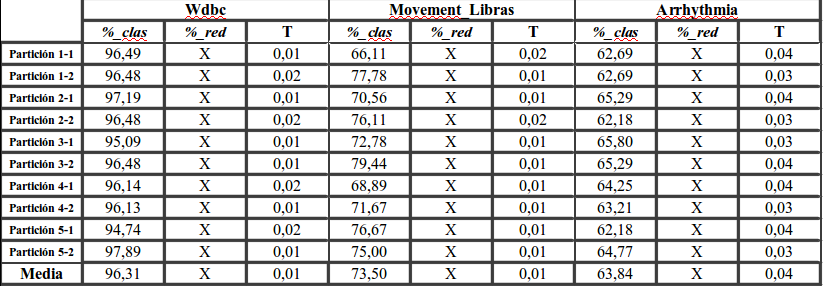
\includegraphics[scale=0.3]{../../../../../../Escritorio/capturas de resultados/3NN.jpg} 
\end{document}